\documentclass[]{article}
\usepackage{lmodern}
\usepackage{amssymb,amsmath}
\usepackage{ifxetex,ifluatex}
\usepackage{fixltx2e} % provides \textsubscript
\ifnum 0\ifxetex 1\fi\ifluatex 1\fi=0 % if pdftex
  \usepackage[T1]{fontenc}
  \usepackage[utf8]{inputenc}
\else % if luatex or xelatex
  \ifxetex
    \usepackage{mathspec}
  \else
    \usepackage{fontspec}
  \fi
  \defaultfontfeatures{Ligatures=TeX,Scale=MatchLowercase}
\fi
% use upquote if available, for straight quotes in verbatim environments
\IfFileExists{upquote.sty}{\usepackage{upquote}}{}
% use microtype if available
\IfFileExists{microtype.sty}{%
\usepackage{microtype}
\UseMicrotypeSet[protrusion]{basicmath} % disable protrusion for tt fonts
}{}
\usepackage[margin=1in]{geometry}
\usepackage{hyperref}
\hypersetup{unicode=true,
            pdftitle={Curs Biostatistica 2017 - Laborator 3 \& 4},
            pdfborder={0 0 0},
            breaklinks=true}
\urlstyle{same}  % don't use monospace font for urls
\usepackage{color}
\usepackage{fancyvrb}
\newcommand{\VerbBar}{|}
\newcommand{\VERB}{\Verb[commandchars=\\\{\}]}
\DefineVerbatimEnvironment{Highlighting}{Verbatim}{commandchars=\\\{\}}
% Add ',fontsize=\small' for more characters per line
\usepackage{framed}
\definecolor{shadecolor}{RGB}{248,248,248}
\newenvironment{Shaded}{\begin{snugshade}}{\end{snugshade}}
\newcommand{\KeywordTok}[1]{\textcolor[rgb]{0.13,0.29,0.53}{\textbf{{#1}}}}
\newcommand{\DataTypeTok}[1]{\textcolor[rgb]{0.13,0.29,0.53}{{#1}}}
\newcommand{\DecValTok}[1]{\textcolor[rgb]{0.00,0.00,0.81}{{#1}}}
\newcommand{\BaseNTok}[1]{\textcolor[rgb]{0.00,0.00,0.81}{{#1}}}
\newcommand{\FloatTok}[1]{\textcolor[rgb]{0.00,0.00,0.81}{{#1}}}
\newcommand{\ConstantTok}[1]{\textcolor[rgb]{0.00,0.00,0.00}{{#1}}}
\newcommand{\CharTok}[1]{\textcolor[rgb]{0.31,0.60,0.02}{{#1}}}
\newcommand{\SpecialCharTok}[1]{\textcolor[rgb]{0.00,0.00,0.00}{{#1}}}
\newcommand{\StringTok}[1]{\textcolor[rgb]{0.31,0.60,0.02}{{#1}}}
\newcommand{\VerbatimStringTok}[1]{\textcolor[rgb]{0.31,0.60,0.02}{{#1}}}
\newcommand{\SpecialStringTok}[1]{\textcolor[rgb]{0.31,0.60,0.02}{{#1}}}
\newcommand{\ImportTok}[1]{{#1}}
\newcommand{\CommentTok}[1]{\textcolor[rgb]{0.56,0.35,0.01}{\textit{{#1}}}}
\newcommand{\DocumentationTok}[1]{\textcolor[rgb]{0.56,0.35,0.01}{\textbf{\textit{{#1}}}}}
\newcommand{\AnnotationTok}[1]{\textcolor[rgb]{0.56,0.35,0.01}{\textbf{\textit{{#1}}}}}
\newcommand{\CommentVarTok}[1]{\textcolor[rgb]{0.56,0.35,0.01}{\textbf{\textit{{#1}}}}}
\newcommand{\OtherTok}[1]{\textcolor[rgb]{0.56,0.35,0.01}{{#1}}}
\newcommand{\FunctionTok}[1]{\textcolor[rgb]{0.00,0.00,0.00}{{#1}}}
\newcommand{\VariableTok}[1]{\textcolor[rgb]{0.00,0.00,0.00}{{#1}}}
\newcommand{\ControlFlowTok}[1]{\textcolor[rgb]{0.13,0.29,0.53}{\textbf{{#1}}}}
\newcommand{\OperatorTok}[1]{\textcolor[rgb]{0.81,0.36,0.00}{\textbf{{#1}}}}
\newcommand{\BuiltInTok}[1]{{#1}}
\newcommand{\ExtensionTok}[1]{{#1}}
\newcommand{\PreprocessorTok}[1]{\textcolor[rgb]{0.56,0.35,0.01}{\textit{{#1}}}}
\newcommand{\AttributeTok}[1]{\textcolor[rgb]{0.77,0.63,0.00}{{#1}}}
\newcommand{\RegionMarkerTok}[1]{{#1}}
\newcommand{\InformationTok}[1]{\textcolor[rgb]{0.56,0.35,0.01}{\textbf{\textit{{#1}}}}}
\newcommand{\WarningTok}[1]{\textcolor[rgb]{0.56,0.35,0.01}{\textbf{\textit{{#1}}}}}
\newcommand{\AlertTok}[1]{\textcolor[rgb]{0.94,0.16,0.16}{{#1}}}
\newcommand{\ErrorTok}[1]{\textcolor[rgb]{0.64,0.00,0.00}{\textbf{{#1}}}}
\newcommand{\NormalTok}[1]{{#1}}
\usepackage{longtable,booktabs}
\usepackage{graphicx,grffile}
\makeatletter
\def\maxwidth{\ifdim\Gin@nat@width>\linewidth\linewidth\else\Gin@nat@width\fi}
\def\maxheight{\ifdim\Gin@nat@height>\textheight\textheight\else\Gin@nat@height\fi}
\makeatother
% Scale images if necessary, so that they will not overflow the page
% margins by default, and it is still possible to overwrite the defaults
% using explicit options in \includegraphics[width, height, ...]{}
\setkeys{Gin}{width=\maxwidth,height=\maxheight,keepaspectratio}
\IfFileExists{parskip.sty}{%
\usepackage{parskip}
}{% else
\setlength{\parindent}{0pt}
\setlength{\parskip}{6pt plus 2pt minus 1pt}
}
\setlength{\emergencystretch}{3em}  % prevent overfull lines
\providecommand{\tightlist}{%
  \setlength{\itemsep}{0pt}\setlength{\parskip}{0pt}}
\setcounter{secnumdepth}{5}
% Redefines (sub)paragraphs to behave more like sections
\ifx\paragraph\undefined\else
\let\oldparagraph\paragraph
\renewcommand{\paragraph}[1]{\oldparagraph{#1}\mbox{}}
\fi
\ifx\subparagraph\undefined\else
\let\oldsubparagraph\subparagraph
\renewcommand{\subparagraph}[1]{\oldsubparagraph{#1}\mbox{}}
\fi

%%% Use protect on footnotes to avoid problems with footnotes in titles
\let\rmarkdownfootnote\footnote%
\def\footnote{\protect\rmarkdownfootnote}

%%% Change title format to be more compact
\usepackage{titling}

% Create subtitle command for use in maketitle
\newcommand{\subtitle}[1]{
  \posttitle{
    \begin{center}\large#1\end{center}
    }
}

\setlength{\droptitle}{-2em}
  \title{Curs Biostatistica 2017 - Laborator 3 \& 4}
  \pretitle{\vspace{\droptitle}\centering\huge}
  \posttitle{\par}
  \author{}
  \preauthor{}\postauthor{}
  \date{}
  \predate{}\postdate{}

\usepackage{booktabs}
\usepackage{longtable}
\usepackage{framed,color}
\definecolor{shadecolor}{RGB}{248,248,248}

\ifxetex
  \usepackage{letltxmacro}
  \setlength{\XeTeXLinkMargin}{1pt}
  \LetLtxMacro\SavedIncludeGraphics\includegraphics
  \def\includegraphics#1#{% #1 catches optional stuff (star/opt. arg.)
    \IncludeGraphicsAux{#1}%
  }%
  \newcommand*{\IncludeGraphicsAux}[2]{%
    \XeTeXLinkBox{%
      \SavedIncludeGraphics#1{#2}%
    }%
  }%
\fi

\newenvironment{rmdblock}[1]
  {\begin{shaded*}
  \begin{itemize}
  \renewcommand{\labelitemi}{
    \raisebox{-.7\height}[0pt][0pt]{
      {\setkeys{Gin}{width=2em,keepaspectratio}\includegraphics{images/icons/#1}}
    }
  }
  \item
  }
  {
  \end{itemize}
  \end{shaded*}
  }
\newenvironment{rmdcaution}
  {\begin{rmdblock}{caution}}
  {\end{rmdblock}}
\newenvironment{rmdinsight}
  {\begin{rmdblock}{insight}}
  {\end{rmdblock}}
\newenvironment{rmdexercise}
  {\begin{rmdblock}{exercise}}
  {\end{rmdblock}}
\newenvironment{rmdtip}
  {\begin{rmdblock}{tip}}
  {\end{rmdblock}}

\begin{document}
\maketitle

{
\setcounter{tocdepth}{2}
\tableofcontents
}
\section{\texorpdfstring{Compararea proporțiilor, tabele de contingență
\(2\times2\)}{Compararea proporțiilor, tabele de contingență 2\textbackslash{}times2}}\label{compararea-proportiilor-tabele-de-contingenta-2times2}

\begin{center}\rule{0.5\linewidth}{\linethickness}\end{center}

\subsection{Aproximarea normală}\label{aproximarea-normala}

\begin{center}\rule{0.5\linewidth}{\linethickness}\end{center}

\begin{quote}
Un studiu clinic a investigat efectele metodelor contraceptive orale
(OC) asupra bolilor de inimă la femeile cu vârste între 40 și 44 de ani.
Cercetătorii au găsit că printre 5000 de femei care utilizau metode
contraceptive orale la momentul studiului (cazuri), 13 dintre acestea au
dezvoltat un infarct miocardic (MI) (pe o perioadă de 3 ani) pe când
printre 10000 de femei care nu au folosit niciodată OC (grupul de
control) doar 7 au dezvoltat MI (pe aceeași perioadă). Vrem să vedem
dacă există vreo asociere între consumul de anticoncepționale pe cale
orală și incidența infarctului miocardic (pe această perioadă).
\end{quote}

Dacă notăm cu \(p_1=\mathbb{P}(MI\,|\,OC)\) și
\(p_2=\mathbb{P}(MI\,|\,non-OC)\) atunci vrem să testăm:

\[
  \begin{array}{ll}
    H_0:\,\,p_1=p_2\\
    H_1:\,\,p_1\neq p_2
  \end{array}
\]

\begin{Shaded}
\begin{Highlighting}[]
\NormalTok{n1 =}\StringTok{ }\DecValTok{5000} \CommentTok{# nr total cazuri OC}
\NormalTok{n11 =}\StringTok{ }\DecValTok{13} \CommentTok{# nr cazuri cu MI}

\NormalTok{n2 =}\StringTok{ }\DecValTok{10000} \CommentTok{# nr total control non-OC}
\NormalTok{n21 =}\StringTok{ }\DecValTok{7} \CommentTok{# nr control cu MI}

\NormalTok{p1 =}\StringTok{ }\NormalTok{n11/n1}
\NormalTok{p2 =}\StringTok{ }\NormalTok{n21/n2}

\NormalTok{p =}\StringTok{ }\NormalTok{(n11+n21)/(n1+n2) }\CommentTok{# proportia comuna - pooled p}

\CommentTok{# Verificam daca putem aplica aproximarea normala }
\NormalTok{n1*p*(}\DecValTok{1}\NormalTok{-p)>}\DecValTok{5}
\end{Highlighting}
\end{Shaded}

\begin{verbatim}
## [1] TRUE
\end{verbatim}

\begin{Shaded}
\begin{Highlighting}[]
\NormalTok{n2*p*(}\DecValTok{1}\NormalTok{-p)>}\DecValTok{5}
\end{Highlighting}
\end{Shaded}

\begin{verbatim}
## [1] TRUE
\end{verbatim}

\begin{Shaded}
\begin{Highlighting}[]
\CommentTok{# Calculam statistica de test cu corectia de continuitate}
\NormalTok{z =}\StringTok{ }\NormalTok{(}\KeywordTok{abs}\NormalTok{(p1-p2)-}\FloatTok{0.5}\NormalTok{*(}\DecValTok{1}\NormalTok{/n1}\DecValTok{+1}\NormalTok{/n2))/}\KeywordTok{sqrt}\NormalTok{(p*(}\DecValTok{1}\NormalTok{-p)*(}\DecValTok{1}\NormalTok{/n1}\DecValTok{+1}\NormalTok{/n2))}
\NormalTok{z}
\end{Highlighting}
\end{Shaded}

\begin{verbatim}
## [1] 2.768839
\end{verbatim}

\begin{Shaded}
\begin{Highlighting}[]
\CommentTok{# Calcul de p-valoare: test bilateral}
\NormalTok{pval =}\StringTok{ }\KeywordTok{min}\NormalTok{(}\DecValTok{2}\NormalTok{*(}\DecValTok{1}\NormalTok{-}\KeywordTok{pnorm}\NormalTok{(z)),}\DecValTok{1}\NormalTok{)}
\NormalTok{pval}
\end{Highlighting}
\end{Shaded}

\begin{verbatim}
## [1] 0.005625635
\end{verbatim}

\begin{Shaded}
\begin{Highlighting}[]
\CommentTok{# Intervalul de incredere}

\KeywordTok{cat}\NormalTok{(}\StringTok{"IC pentru p1-p2 la pragul de semnificatie 95% este }\CharTok{\textbackslash{}n}\StringTok{"}\NormalTok{,}
    \StringTok{"IC = ["}\NormalTok{, p1-p2 -}\StringTok{ }\KeywordTok{qnorm}\NormalTok{(}\FloatTok{0.975}\NormalTok{) *}\KeywordTok{sqrt}\NormalTok{(p*(}\DecValTok{1}\NormalTok{-p)*(}\DecValTok{1}\NormalTok{/n1}\DecValTok{+1}\NormalTok{/n2)), }\StringTok{","}\NormalTok{, }
    \NormalTok{p1-p2 +}\StringTok{ }\KeywordTok{qnorm}\NormalTok{(}\FloatTok{0.9755}\NormalTok{) *}\KeywordTok{sqrt}\NormalTok{(p*(}\DecValTok{1}\NormalTok{-p)*(}\DecValTok{1}\NormalTok{/n1}\DecValTok{+1}\NormalTok{/n2)),}\StringTok{"]"}\NormalTok{)}
\end{Highlighting}
\end{Shaded}

\begin{verbatim}
## IC pentru p1-p2 la pragul de semnificatie 95% este 
##  IC = [ 0.0006612366 , 0.003144216 ]
\end{verbatim}

\begin{Shaded}
\begin{Highlighting}[]
\CommentTok{# Intervalul de incredere Agresti & Caffo 2000}

\NormalTok{p1b =}\StringTok{ }\NormalTok{(n11}\DecValTok{+1}\NormalTok{)/(n1}\DecValTok{+2}\NormalTok{)}
\NormalTok{p2b =}\StringTok{ }\NormalTok{(n21}\DecValTok{+1}\NormalTok{)/(n2}\DecValTok{+2}\NormalTok{)}

\KeywordTok{cat}\NormalTok{(}\StringTok{"IC (Agresti-Caffo) pentru p1-p2 la pragul de semnificatie 95% este }\CharTok{\textbackslash{}n}\StringTok{"}\NormalTok{,}
    \StringTok{"IC = ["}\NormalTok{, p1b-p2b -}\StringTok{ }\KeywordTok{qnorm}\NormalTok{(}\FloatTok{0.975}\NormalTok{) *}\KeywordTok{sqrt}\NormalTok{(p1b*(}\DecValTok{1}\NormalTok{-p1b)/(n1}\DecValTok{+2}\NormalTok{)+p2b*(}\DecValTok{1}\NormalTok{-p2b)/(n2}\DecValTok{+2}\NormalTok{)), }\StringTok{","}\NormalTok{,}
    \NormalTok{p1b-p2b +}\StringTok{ }\KeywordTok{qnorm}\NormalTok{(}\FloatTok{0.975}\NormalTok{) *}\KeywordTok{sqrt}\NormalTok{(p1b*(}\DecValTok{1}\NormalTok{-p1b)/(n1}\DecValTok{+2}\NormalTok{)+p2b*(}\DecValTok{1}\NormalTok{-p2b)/(n2}\DecValTok{+2}\NormalTok{)),}\StringTok{"]"}\NormalTok{)}
\end{Highlighting}
\end{Shaded}

\begin{verbatim}
## IC (Agresti-Caffo) pentru p1-p2 la pragul de semnificatie 95% este 
##  IC = [ 0.0004336558 , 0.003564425 ]
\end{verbatim}

\begin{center}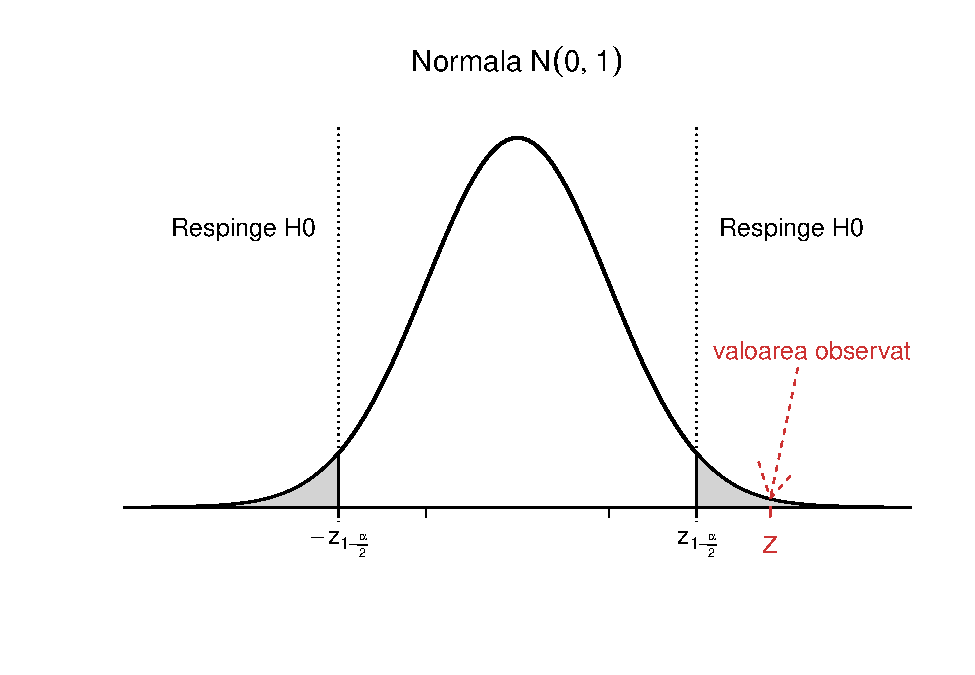
\includegraphics[width=0.9\linewidth]{Lab_3_files/figure-latex/unnamed-chunk-2-1} \end{center}

Concluzionăm că folosirea de anticoncepționale pe cale orală este
semnificativ asociat cu incidența crescută de cazuri de MI pe perioada
de 3 ani. Puteți crea o funcție care să automatizeze procesul ?

\subsection{\texorpdfstring{Pearson
\(\chi^2\)}{Pearson \textbackslash{}chi\^{}2}}\label{pearson-chi2}

\begin{center}\rule{0.5\linewidth}{\linethickness}\end{center}

Considerăm aceeași problemă de mai sus dar o scriem sub formă de tabel
de contingență \(2\times2\) (tabelul observat):

\begin{longtable}[]{@{}lccc@{}}
\toprule
& MI & non-MI & Total\tabularnewline
\midrule
\endhead
OC & 13 & 4987 & 5000\tabularnewline
non-OC & 7 & 9993 & 10000\tabularnewline
Total & 20 & 14980 & 15000\tabularnewline
\bottomrule
\end{longtable}

Calculul tabelului de pe care ne așteptăm să-l observăm
(\(E_{ij}=\frac{n_{i\cdot}n_{\cdot j}}{n}\)):

\begin{Shaded}
\begin{Highlighting}[]
\CommentTok{# Observat}
\NormalTok{n11 =}\StringTok{ }\DecValTok{13}
\NormalTok{n1o =}\StringTok{ }\DecValTok{5000}
\NormalTok{n12 =}\StringTok{ }\NormalTok{n1o-n11}

\NormalTok{n21 =}\StringTok{ }\DecValTok{7}
\NormalTok{n2o =}\StringTok{ }\DecValTok{10000}
\NormalTok{n22 =}\StringTok{ }\NormalTok{n2o-n21}

\NormalTok{no1 =}\StringTok{ }\NormalTok{n11+n21}
\NormalTok{no2 =}\StringTok{ }\NormalTok{n12+n22}

\NormalTok{n =}\StringTok{ }\NormalTok{n1o+n2o}

\CommentTok{#Asteptat}
\NormalTok{e11 =}\StringTok{ }\NormalTok{n1o*no1/n}
\NormalTok{e12 =}\StringTok{ }\NormalTok{n1o*no2/n}
\NormalTok{e21 =}\StringTok{ }\NormalTok{n2o*no1/n}
\NormalTok{e22 =}\StringTok{ }\NormalTok{n2o*no2/n}

\NormalTok{Mobs =}\StringTok{ }\KeywordTok{matrix}\NormalTok{(}\KeywordTok{c}\NormalTok{(n11,n12,n21,n22),}\DataTypeTok{ncol =} \DecValTok{2}\NormalTok{, }\DataTypeTok{byrow =} \NormalTok{T, }
              \DataTypeTok{dimnames =} \KeywordTok{list}\NormalTok{(}\KeywordTok{c}\NormalTok{(}\StringTok{"OC"}\NormalTok{,}\StringTok{"non-OC"}\NormalTok{), }\KeywordTok{c}\NormalTok{(}\StringTok{"MI"}\NormalTok{, }\StringTok{"non-MI"}\NormalTok{)))}

\NormalTok{Mexp =}\StringTok{ }\KeywordTok{matrix}\NormalTok{(}\KeywordTok{c}\NormalTok{(e11,e12,e21,e22),}\DataTypeTok{ncol =} \DecValTok{2}\NormalTok{, }\DataTypeTok{byrow =} \NormalTok{T, }
              \DataTypeTok{dimnames =} \KeywordTok{list}\NormalTok{(}\KeywordTok{c}\NormalTok{(}\StringTok{"OC"}\NormalTok{,}\StringTok{"non-OC"}\NormalTok{), }\KeywordTok{c}\NormalTok{(}\StringTok{"MI"}\NormalTok{, }\StringTok{"non-MI"}\NormalTok{)))}
\NormalTok{Mexp}
\end{Highlighting}
\end{Shaded}

\begin{verbatim}
##               MI   non-MI
## OC      6.666667 4993.333
## non-OC 13.333333 9986.667
\end{verbatim}

\begin{longtable}[]{@{}lcc@{}}
\toprule
& MI & non-MI\tabularnewline
\midrule
\endhead
OC & 6.666667 & 4993.333\tabularnewline
non-OC & 13.333333 & 9986.667\tabularnewline
\bottomrule
\end{longtable}

Calculul statisticii de test cu corecția lui Yates:

\[
  X^2 = \sum_{i=1}^{2}\sum_{j=1}^{2}\frac{\left(|O_{ij}-E_{ij}|-0.5\right)^2}{E_{ij}}\sim_{H_0}\chi_1^2
\]

\begin{Shaded}
\begin{Highlighting}[]
\NormalTok{X2 =}\StringTok{ }\NormalTok{(}\KeywordTok{abs}\NormalTok{(n11-e11)-}\FloatTok{0.5}\NormalTok{)^}\DecValTok{2}\NormalTok{/e11 +}\StringTok{ }\NormalTok{(}\KeywordTok{abs}\NormalTok{(n12-e12)-}\FloatTok{0.5}\NormalTok{)^}\DecValTok{2}\NormalTok{/e12 +}\StringTok{ }
\StringTok{  }\NormalTok{(}\KeywordTok{abs}\NormalTok{(n21-e21)-}\FloatTok{0.5}\NormalTok{)^}\DecValTok{2}\NormalTok{/e21 +}\StringTok{ }\NormalTok{(}\KeywordTok{abs}\NormalTok{(n22-e22)-}\FloatTok{0.5}\NormalTok{)^}\DecValTok{2}\NormalTok{/e22}
\NormalTok{X2}
\end{Highlighting}
\end{Shaded}

\begin{verbatim}
## [1] 7.666472
\end{verbatim}

\begin{Shaded}
\begin{Highlighting}[]
\NormalTok{pval =}\StringTok{ }\DecValTok{1}\NormalTok{-}\KeywordTok{pchisq}\NormalTok{(X2,}\DecValTok{1}\NormalTok{) }\CommentTok{#df = 1}
\NormalTok{pval}
\end{Highlighting}
\end{Shaded}

\begin{verbatim}
## [1] 0.005625635
\end{verbatim}

Sau folosind testul lui Pearson cu corecția lui Yates
\texttt{chisq.test} avem:

\begin{Shaded}
\begin{Highlighting}[]
\KeywordTok{chisq.test}\NormalTok{(Mobs)}
\end{Highlighting}
\end{Shaded}

\begin{verbatim}
## 
##  Pearson's Chi-squared test with Yates' continuity correction
## 
## data:  Mobs
## X-squared = 7.6665, df = 1, p-value = 0.005626
\end{verbatim}

\begin{center}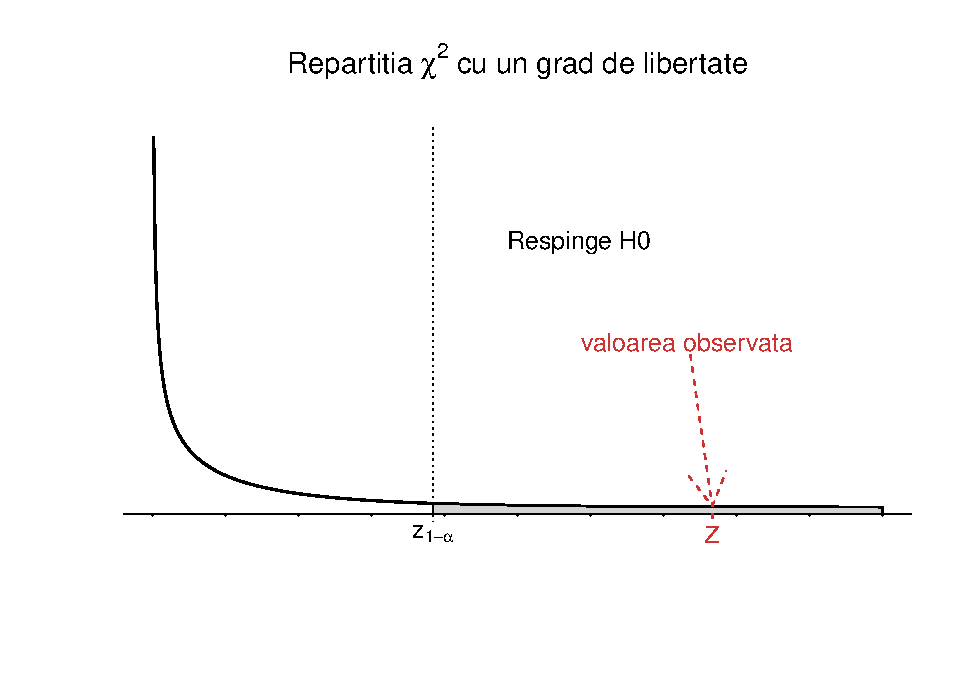
\includegraphics[width=0.9\linewidth]{Lab_3_files/figure-latex/unnamed-chunk-8-1} \end{center}

Același rezultat se obține și dacă folosim testul \texttt{prop.test},
acesta fiind un caz particular al testului hi-pătrat:

\begin{Shaded}
\begin{Highlighting}[]
\KeywordTok{prop.test}\NormalTok{(Mobs)}
\end{Highlighting}
\end{Shaded}

\begin{verbatim}
## 
##  2-sample test for equality of proportions with continuity
##  correction
## 
## data:  Mobs
## X-squared = 7.6665, df = 1, p-value = 0.005626
## alternative hypothesis: two.sided
## 95 percent confidence interval:
##  0.0002463116 0.0035536884
## sample estimates:
## prop 1 prop 2 
## 0.0026 0.0007
\end{verbatim}

\subsection{Raportul de verosimilitate
maximă}\label{raportul-de-verosimilitate-maxima}

\begin{center}\rule{0.5\linewidth}{\linethickness}\end{center}

În contextul exemplului de mai sus vrem să vedem testul bazat pe
raportul de verosimilitate. Considerând modelul multinomial
\((n_{11},n_{12},n_{21},n_{22})\sim \mathcal{M}(n;p_{11},p_{12},p_{21},p_{22})\),
obținem raportul de verosimilitate

\[
  \Lambda(x)=\frac{\sup_{\theta\in\Theta_0}L(\theta|x)}{\sup_{\theta\in\Theta}L(\theta|x)}=\prod_{i=1}^{2}\prod_{j=1}^{2}\left(\frac{n_{i\cdot}\times n_{\cdot j}}{n\times n_{ij}}\right)^{n_{ij}}
\] și din teorema lui Wilks (cazul multidimensional) avem
\(-2\log\Lambda\to\chi^2(d-d_0)\) unde \(d=\dim(\Theta)\) și
\(d_0=\dim(\Theta_0)\). În cazul nostru

\[
  \begin{array}{ll}
    \Theta = \left\{(p_{11},p_{12},p_{21},p_{22})\,|\,p_{ij}\in(0,1),\,\sum_{i=1}^{2}\sum_{j=1}^{2}p_{ij}=1\right\}\\
    \Theta_0 = \left\{(p_{1}q_1,p_{1}q_2,p_{2}q_1,p_{2}q_2)\,|\,p_{i},q_j\in(0,1),\,\sum_{i=1}^{2}p_{i}=1,\,\sum_{j=1}^{2}q_j=1\right\}
  \end{array}
\] unde \(p_i\) și \(q_j\) sunt repartițiile marginale. Obținem că
\(\dim(\Theta)=4-1\) iar \(\dim(\Theta_0)=4-2\), deci
\(-2\log\Lambda\to\chi^2(1)\).

\begin{Shaded}
\begin{Highlighting}[]
\CommentTok{# Observat}
\NormalTok{n11 =}\StringTok{ }\DecValTok{13}
\NormalTok{n1o =}\StringTok{ }\DecValTok{5000}
\NormalTok{n12 =}\StringTok{ }\NormalTok{n1o-n11}

\NormalTok{n21 =}\StringTok{ }\DecValTok{7}
\NormalTok{n2o =}\StringTok{ }\DecValTok{10000}
\NormalTok{n22 =}\StringTok{ }\NormalTok{n2o-n21}

\NormalTok{no1 =}\StringTok{ }\NormalTok{n11+n21}
\NormalTok{no2 =}\StringTok{ }\NormalTok{n12+n22}

\NormalTok{LRT =}\StringTok{ }\NormalTok{n11*}\KeywordTok{log}\NormalTok{((n1o*no1)/(n*n11)) +}\StringTok{ }\NormalTok{n12*}\KeywordTok{log}\NormalTok{((n1o*no2)/(n*n12)) +}\StringTok{ }
\StringTok{  }\NormalTok{n21*}\KeywordTok{log}\NormalTok{((n2o*no1)/(n*n21)) +}\StringTok{ }\NormalTok{n22*}\KeywordTok{log}\NormalTok{((n2o*no2)/(n*n22))}
\NormalTok{LRT =}\StringTok{ }\NormalTok{-}\DecValTok{2}\NormalTok{*LRT}
\NormalTok{LRT}
\end{Highlighting}
\end{Shaded}

\begin{verbatim}
## [1] 8.354617
\end{verbatim}

\begin{Shaded}
\begin{Highlighting}[]
\NormalTok{pval =}\StringTok{ }\DecValTok{1}\NormalTok{-}\KeywordTok{pchisq}\NormalTok{(LRT,}\DecValTok{1}\NormalTok{) }\CommentTok{#df = 1}
\NormalTok{pval}
\end{Highlighting}
\end{Shaded}

\begin{verbatim}
## [1] 0.003847085
\end{verbatim}

\begin{center}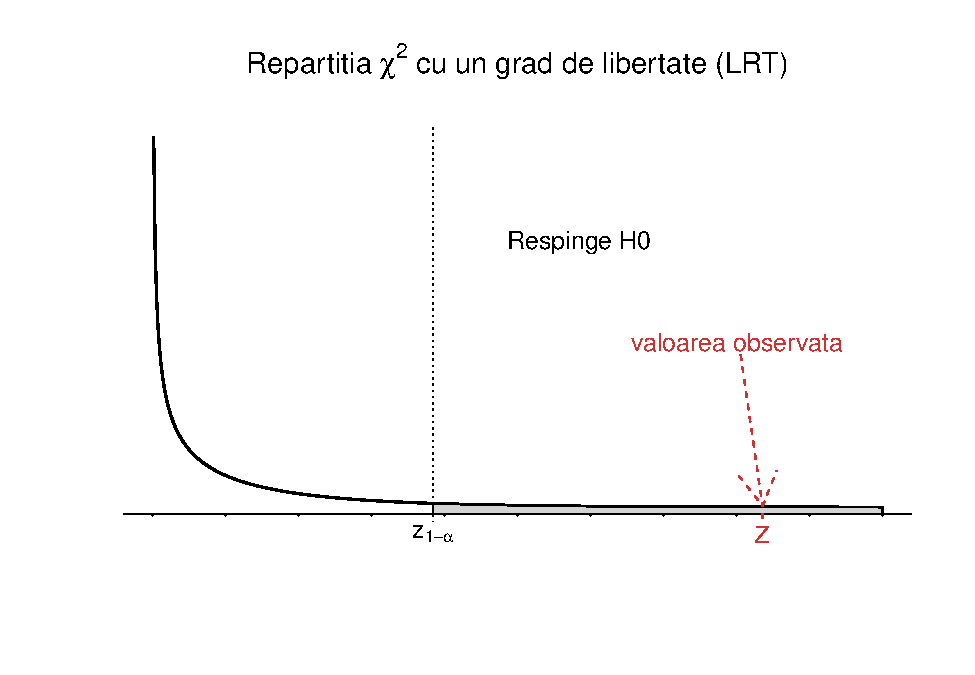
\includegraphics[width=0.9\linewidth]{Lab_3_files/figure-latex/unnamed-chunk-11-1} \end{center}

Să creăm o funcție care automatizează procesul:

\begin{Shaded}
\begin{Highlighting}[]
\NormalTok{LRT1 =}\StringTok{ }\NormalTok{function(dat)\{}
  \CommentTok{# dat este sub forma de matrice }
  \NormalTok{rs =}\StringTok{ }\KeywordTok{rowSums}\NormalTok{(dat) }\CommentTok{# apply(dat, 1, sum)}
  \NormalTok{cs =}\StringTok{ }\KeywordTok{colSums}\NormalTok{(dat) }\CommentTok{# apply(dat, 2, sum)}
  
  \NormalTok{n =}\StringTok{ }\KeywordTok{sum}\NormalTok{(dat)}
  
  \NormalTok{expected <-}\StringTok{ }\KeywordTok{outer}\NormalTok{(rs,cs,}\StringTok{"*"}\NormalTok{)/n}
  
  \NormalTok{lrt <-}\StringTok{ }\NormalTok{-}\DecValTok{2}\NormalTok{*}\KeywordTok{sum}\NormalTok{(dat *}\StringTok{ }\KeywordTok{log}\NormalTok{(expected/dat)) }
  
  \NormalTok{dm =}\StringTok{ }\KeywordTok{dim}\NormalTok{(dat) }\CommentTok{# dimensiunea tabloului pentru a calcula gradele de libertate}
  \NormalTok{pval =}\StringTok{ }\DecValTok{1}\NormalTok{-}\KeywordTok{pchisq}\NormalTok{(lrt,(dm[}\DecValTok{1}\NormalTok{]-}\DecValTok{1}\NormalTok{)*(dm[}\DecValTok{2}\NormalTok{]-}\DecValTok{1}\NormalTok{))}
  
  \KeywordTok{cat}\NormalTok{(}\StringTok{"Statistica LRT este "}\NormalTok{, lrt, }\StringTok{"}\CharTok{\textbackslash{}n}\StringTok{"}\NormalTok{)}
  \KeywordTok{cat}\NormalTok{(}\StringTok{"P-valoarea testului bazat pe raportul de verosimilitate este "}\NormalTok{, pval)}
  
  \KeywordTok{return}\NormalTok{(}\KeywordTok{list}\NormalTok{(}\DataTypeTok{statistic =} \NormalTok{lrt, }\DataTypeTok{pvalue =} \NormalTok{pval))}
\NormalTok{\}}

\NormalTok{Mobs =}\StringTok{ }\KeywordTok{matrix}\NormalTok{(}\KeywordTok{c}\NormalTok{(n11,n12,n21,n22),}\DataTypeTok{ncol =} \DecValTok{2}\NormalTok{, }\DataTypeTok{byrow =} \NormalTok{T, }
              \DataTypeTok{dimnames =} \KeywordTok{list}\NormalTok{(}\KeywordTok{c}\NormalTok{(}\StringTok{"OC"}\NormalTok{,}\StringTok{"non-OC"}\NormalTok{), }\KeywordTok{c}\NormalTok{(}\StringTok{"MI"}\NormalTok{, }\StringTok{"non-MI"}\NormalTok{)))}

\KeywordTok{LRT1}\NormalTok{(Mobs) }
\end{Highlighting}
\end{Shaded}

\begin{verbatim}
## Statistica LRT este  8.354617 
## P-valoarea testului bazat pe raportul de verosimilitate este  0.003847085
\end{verbatim}

\begin{verbatim}
## $statistic
## [1] 8.354617
## 
## $pvalue
## [1] 0.003847085
\end{verbatim}

\subsection{Testul exact al lui
Fisher}\label{testul-exact-al-lui-fisher}

\begin{center}\rule{0.5\linewidth}{\linethickness}\end{center}

\begin{quote}
Să presupunem că vrem să investigăm legătura dintre regimul bogat în
sare și decesul datorat unei boli cardiovasculare (CVD). Să presupunem
că suntem în contextul unui studiu retrospectiv efectuat pe un grup de
bărbați cu vârste cuprinse între 50 și 54 de ani dintr-o anumită regiune
geografică care au decedat pe parcursul unui luni. S-a încercat
introducerea în studiu a unui grup cât mai omogen (s-a încercat
includerea în studiu a unui număr egal de persoane care au decedat din
cauză de CVD și care au decedat din alte cauze). S-a obținut următorul
tabel:
\end{quote}

\begin{longtable}[]{@{}lccc@{}}
\toprule
& Ridicat Sare & Scazut Sare & Total\tabularnewline
\midrule
\endhead
non-CVD & 2 & 23 & 25\tabularnewline
CVD & 5 & 30 & 35\tabularnewline
Total & 7 & 53 & 60\tabularnewline
\bottomrule
\end{longtable}

Tabelul pe care ne așteptam să-l obținem (\(H_0\)) este:

\begin{Shaded}
\begin{Highlighting}[]
\CommentTok{# Observat}
\NormalTok{n11 =}\StringTok{ }\DecValTok{2}
\NormalTok{n1o =}\StringTok{ }\DecValTok{25}
\NormalTok{n12 =}\StringTok{ }\NormalTok{n1o-n11}

\NormalTok{n21 =}\StringTok{ }\DecValTok{5}
\NormalTok{n2o =}\StringTok{ }\DecValTok{35}
\NormalTok{n22 =}\StringTok{ }\NormalTok{n2o-n21}

\NormalTok{no1 =}\StringTok{ }\NormalTok{n11+n21}
\NormalTok{no2 =}\StringTok{ }\NormalTok{n12+n22}

\NormalTok{n =}\StringTok{ }\NormalTok{n1o+n2o}

\CommentTok{#Asteptat}
\NormalTok{e11 =}\StringTok{ }\NormalTok{n1o*no1/n}
\NormalTok{e12 =}\StringTok{ }\NormalTok{n1o*no2/n}
\NormalTok{e21 =}\StringTok{ }\NormalTok{n2o*no1/n}
\NormalTok{e22 =}\StringTok{ }\NormalTok{n2o*no2/n}

\NormalTok{MobsF =}\StringTok{ }\KeywordTok{matrix}\NormalTok{(}\KeywordTok{c}\NormalTok{(n11,n12,n21,n22),}\DataTypeTok{ncol =} \DecValTok{2}\NormalTok{, }\DataTypeTok{byrow =} \NormalTok{T, }
               \DataTypeTok{dimnames =} \KeywordTok{list}\NormalTok{(}\KeywordTok{c}\NormalTok{(}\StringTok{"non-CVD"}\NormalTok{, }\StringTok{"CVD"}\NormalTok{), }\KeywordTok{c}\NormalTok{(}\StringTok{"Ridicat Sare"}\NormalTok{, }\StringTok{"Scazut Sare"}\NormalTok{)))}

\NormalTok{MexpF =}\StringTok{ }\KeywordTok{matrix}\NormalTok{(}\KeywordTok{c}\NormalTok{(e11,e12,e21,e22),}\DataTypeTok{ncol =} \DecValTok{2}\NormalTok{, }\DataTypeTok{byrow =} \NormalTok{T, }
               \DataTypeTok{dimnames =} \KeywordTok{list}\NormalTok{(}\KeywordTok{c}\NormalTok{(}\StringTok{"non-CVD"}\NormalTok{, }\StringTok{"CVD"}\NormalTok{), }\KeywordTok{c}\NormalTok{(}\StringTok{"Ridicat Sare"}\NormalTok{, }\StringTok{"Scazut Sare"}\NormalTok{)))}
\NormalTok{MexpF}
\end{Highlighting}
\end{Shaded}

\begin{verbatim}
##         Ridicat Sare Scazut Sare
## non-CVD     2.916667    22.08333
## CVD         4.083333    30.91667
\end{verbatim}

\begin{longtable}[]{@{}lcc@{}}
\toprule
& Ridicat Sare & Scazut Sare\tabularnewline
\midrule
\endhead
non-CVD & 2.916667 & 22.08333\tabularnewline
CVD & 4.083333 & 30.91667\tabularnewline
\bottomrule
\end{longtable}

Observăm că avem două celule în tabelul așteptat care conțin mai puțin
de 5 observații prin urmare nu putem folosi metodele de mai sus
(aproximarea normală, testul lui Pearson sau testul bazat pe raportul de
verosimilitate). Dacă am încerca am obține:

\begin{Shaded}
\begin{Highlighting}[]
\CommentTok{# Testul lui Pearson (Hi patrat)}

\KeywordTok{chisq.test}\NormalTok{(MobsF)}
\end{Highlighting}
\end{Shaded}

\begin{verbatim}
## Warning in chisq.test(MobsF): Chi-squared approximation may be incorrect
\end{verbatim}

\begin{verbatim}
## 
##  Pearson's Chi-squared test with Yates' continuity correction
## 
## data:  MobsF
## X-squared = 0.11552, df = 1, p-value = 0.7339
\end{verbatim}

\begin{Shaded}
\begin{Highlighting}[]
\CommentTok{# Testul bazat pe raportul de verosimilitate}

\KeywordTok{LRT1}\NormalTok{(MobsF)}
\end{Highlighting}
\end{Shaded}

\begin{verbatim}
## Statistica LRT este  0.5810517 
## P-valoarea testului bazat pe raportul de verosimilitate este  0.4459004
\end{verbatim}

\begin{verbatim}
## $statistic
## [1] 0.5810517
## 
## $pvalue
## [1] 0.4459004
\end{verbatim}

Enumerăm tabelele și probabilitățile lor de apariție:

\begin{Shaded}
\begin{Highlighting}[]
\CommentTok{# Fixez marginalele}

\NormalTok{n1o =}\StringTok{ }\DecValTok{25}
\NormalTok{n2o =}\StringTok{ }\DecValTok{35}
  
\NormalTok{no1 =}\StringTok{ }\DecValTok{7}
\NormalTok{no2 =}\StringTok{ }\DecValTok{53}

\NormalTok{for (i in }\DecValTok{0}\NormalTok{:}\DecValTok{7}\NormalTok{)\{}
  \KeywordTok{cat}\NormalTok{(}\StringTok{"-------------------------------------}\CharTok{\textbackslash{}n}\StringTok{"}\NormalTok{)}
  \KeywordTok{cat}\NormalTok{(}\StringTok{"Tabelul "}\NormalTok{, i}\DecValTok{+1}\NormalTok{, }\StringTok{" :}\CharTok{\textbackslash{}n}\StringTok{"}\NormalTok{)}
  
  \CommentTok{# calculez valorile din tabel}
  \NormalTok{n11 =}\StringTok{ }\NormalTok{i}
  \NormalTok{n12 =}\StringTok{ }\NormalTok{n1o -}\StringTok{ }\NormalTok{n11}
  \NormalTok{n21 =}\StringTok{ }\NormalTok{no1 -}\StringTok{ }\NormalTok{n11}
  \NormalTok{n22 =}\StringTok{ }\NormalTok{no2 -}\StringTok{ }\NormalTok{n12}
  
  \NormalTok{MobsF1 =}\StringTok{ }\KeywordTok{matrix}\NormalTok{(}\KeywordTok{c}\NormalTok{(n11,n12,n21,n22),}\DataTypeTok{ncol =} \DecValTok{2}\NormalTok{, }\DataTypeTok{byrow =} \NormalTok{T, }
                  \DataTypeTok{dimnames =} \KeywordTok{list}\NormalTok{(}\KeywordTok{c}\NormalTok{(}\StringTok{"non-CVD"}\NormalTok{, }\StringTok{"CVD"}\NormalTok{), }\KeywordTok{c}\NormalTok{(}\StringTok{"Ridicat Sare"}\NormalTok{, }\StringTok{"Scazut Sare"}\NormalTok{)))}
  
  \KeywordTok{print}\NormalTok{(MobsF1)}
  
  \KeywordTok{cat}\NormalTok{(}\StringTok{"Probabilitatea de a obtine tabelul "}\NormalTok{, i}\DecValTok{+1}\NormalTok{, }\StringTok{" este "}\NormalTok{, }
      \KeywordTok{dhyper}\NormalTok{(i, no1, no2, n1o), }\StringTok{"}\CharTok{\textbackslash{}n}\StringTok{"}\NormalTok{)}
  \KeywordTok{cat}\NormalTok{(}\StringTok{"-------------------------------------}\CharTok{\textbackslash{}n}\StringTok{"}\NormalTok{)}
\NormalTok{\}}
\end{Highlighting}
\end{Shaded}

\begin{verbatim}
## -------------------------------------
## Tabelul  1  :
##         Ridicat Sare Scazut Sare
## non-CVD            0          25
## CVD                7          28
## Probabilitatea de a obtine tabelul  1  este  0.0174117 
## -------------------------------------
## -------------------------------------
## Tabelul  2  :
##         Ridicat Sare Scazut Sare
## non-CVD            1          24
## CVD                6          29
## Probabilitatea de a obtine tabelul  2  este  0.1050706 
## -------------------------------------
## -------------------------------------
## Tabelul  3  :
##         Ridicat Sare Scazut Sare
## non-CVD            2          23
## CVD                5          30
## Probabilitatea de a obtine tabelul  3  este  0.2521695 
## -------------------------------------
## -------------------------------------
## Tabelul  4  :
##         Ridicat Sare Scazut Sare
## non-CVD            3          22
## CVD                4          31
## Probabilitatea de a obtine tabelul  4  este  0.3118225 
## -------------------------------------
## -------------------------------------
## Tabelul  5  :
##         Ridicat Sare Scazut Sare
## non-CVD            4          21
## CVD                3          32
## Probabilitatea de a obtine tabelul  5  este  0.214378 
## -------------------------------------
## -------------------------------------
## Tabelul  6  :
##         Ridicat Sare Scazut Sare
## non-CVD            5          20
## CVD                2          33
## Probabilitatea de a obtine tabelul  6  este  0.0818534 
## -------------------------------------
## -------------------------------------
## Tabelul  7  :
##         Ridicat Sare Scazut Sare
## non-CVD            6          19
## CVD                1          34
## Probabilitatea de a obtine tabelul  7  este  0.01604969 
## -------------------------------------
## -------------------------------------
## Tabelul  8  :
##         Ridicat Sare Scazut Sare
## non-CVD            7          18
## CVD                0          35
## Probabilitatea de a obtine tabelul  8  este  0.00124467 
## -------------------------------------
\end{verbatim}

Aplicăm testul exact al lui Fisher \texttt{fisher.test}:

\begin{Shaded}
\begin{Highlighting}[]
\KeywordTok{fisher.test}\NormalTok{(MobsF)}
\end{Highlighting}
\end{Shaded}

\begin{verbatim}
## 
##  Fisher's Exact Test for Count Data
## 
## data:  MobsF
## p-value = 0.6882
## alternative hypothesis: true odds ratio is not equal to 1
## 95 percent confidence interval:
##  0.04625243 3.58478157
## sample estimates:
## odds ratio 
##   0.527113
\end{verbatim}

P-valoarea în \texttt{R} este calculată după formula:

\[
  p_{value} = \sum_{\{i:\mathbb{P}(i)\leq \mathbb{P}(obs)\}}\mathbb{P}(i)
\] care în cazul nostru devine

\begin{Shaded}
\begin{Highlighting}[]
\NormalTok{n1o =}\StringTok{ }\DecValTok{25}
\NormalTok{n2o =}\StringTok{ }\DecValTok{35}
  
\NormalTok{no1 =}\StringTok{ }\DecValTok{7}
\NormalTok{no2 =}\StringTok{ }\DecValTok{53}

\NormalTok{n11 =}\StringTok{ }\DecValTok{2}
  
\NormalTok{ps =}\StringTok{ }\KeywordTok{dhyper}\NormalTok{(}\DecValTok{0}\NormalTok{:no1, no1, no2, n1o)}
\NormalTok{pobs =}\StringTok{ }\KeywordTok{dhyper}\NormalTok{(n11, no1, no2, n1o)}

\NormalTok{pval =}\StringTok{ }\KeywordTok{sum}\NormalTok{(ps[ps<=pobs])}
\NormalTok{pval}
\end{Highlighting}
\end{Shaded}

\begin{verbatim}
## [1] 0.6881775
\end{verbatim}

\subsection{Date pereche - Testul lui
McNemar}\label{date-pereche---testul-lui-mcnemar}

\begin{center}\rule{0.5\linewidth}{\linethickness}\end{center}

\begin{quote}
Ne propunem să comparăm două regimuri de chimioterapie pentru pacienții
cu cancer la sân care au efectuat operația de mastectomie. Cele două
grupuri de tratament investigate ar trebui să fie cât mai comparabile
din punct de vedere al celorlalți factori. Presupunem că un studiu de
potrivire (matched study) a fost pregătit așa încât din fiecare pereche
(potrivită din punct de vedere al vârstei și a condițiilor clinice) s-a
selectat aleator un membru căruia i-a fost administrat tratamentul A iar
celuilalt membru tratamentul B. Pacienții au fost urmăriți pe o perioadă
de 5 ani, iar variabila de interes a fost supraviețuirea în această
perioadă. S-au obșinut următoarele date:
\end{quote}

\begin{longtable}[]{@{}lccc@{}}
\toprule
& Supravietuit & Decedat & Total\tabularnewline
\midrule
\endhead
A & 526 & 95 & 621\tabularnewline
B & 515 & 106 & 621\tabularnewline
Total & 1041 & 201 & 1242\tabularnewline
\bottomrule
\end{longtable}

Observăm că nu putem folosi testul lui Pearson (cu corecția lui Yates)
deoarece datele nu sunt \emph{independente}. Dacă am folosi am obține:

\begin{Shaded}
\begin{Highlighting}[]
\NormalTok{M1csq =}\StringTok{ }\KeywordTok{matrix}\NormalTok{(}\KeywordTok{c}\NormalTok{(}\DecValTok{526}\NormalTok{,}\DecValTok{95}\NormalTok{,}\DecValTok{515}\NormalTok{,}\DecValTok{106}\NormalTok{),}\DataTypeTok{ncol =} \DecValTok{2}\NormalTok{, }\DataTypeTok{byrow =} \NormalTok{T)}
\KeywordTok{chisq.test}\NormalTok{(M1csq)}
\end{Highlighting}
\end{Shaded}

\begin{verbatim}
## 
##  Pearson's Chi-squared test with Yates' continuity correction
## 
## data:  M1csq
## X-squared = 0.59357, df = 1, p-value = 0.441
\end{verbatim}

Construim următorul tabel, în care unitatea de analiză nu mai este
\emph{pacientul} ci \emph{perechea} iar perechile sunt clasificate după
cum membrii acelei perechi au supraviețuit sau nu o perioadă
post-operatorie de 5 ani (liniile tabelului sunt rezultatele pacientului
care a urmat tratamentul A iar coloanele sunt rezultatele pacientului
care a urmat tratamentul B):

\begin{longtable}[]{@{}lccc@{}}
\toprule
& Supravietuit & Decedat & Total\tabularnewline
\midrule
\endhead
Supravietuit & 510 & 16 & 526\tabularnewline
Decedat & 5 & 90 & 95\tabularnewline
Total & 515 & 106 & 621\tabularnewline
\bottomrule
\end{longtable}

Observăm că 600 (510+90) de perechi au avut același rezultat (perechi
concordante) și doar 21 de perechi au avut rezultate diferite (perechi
neconcordante).

Aplicăm testul lui McNemar \texttt{mcnemar.test} :

\begin{Shaded}
\begin{Highlighting}[]
\NormalTok{M1 =}\StringTok{ }\KeywordTok{matrix}\NormalTok{(}\KeywordTok{c}\NormalTok{(}\DecValTok{510}\NormalTok{,}\DecValTok{16}\NormalTok{,}\DecValTok{5}\NormalTok{,}\DecValTok{90}\NormalTok{),}\DataTypeTok{ncol =} \DecValTok{2}\NormalTok{, }\DataTypeTok{byrow =} \NormalTok{T, }
           \DataTypeTok{dimnames =} \KeywordTok{list}\NormalTok{(}\KeywordTok{c}\NormalTok{(}\StringTok{"Supravietuit"}\NormalTok{, }\StringTok{"Decedat"}\NormalTok{), }
                           \KeywordTok{c}\NormalTok{(}\StringTok{"Supravietuit"}\NormalTok{, }\StringTok{"Decedat"}\NormalTok{)))}
\KeywordTok{mcnemar.test}\NormalTok{(M1)}
\end{Highlighting}
\end{Shaded}

\begin{verbatim}
## 
##  McNemar's Chi-squared test with continuity correction
## 
## data:  M1
## McNemar's chi-squared = 4.7619, df = 1, p-value = 0.0291
\end{verbatim}

\section{\texorpdfstring{Tabele de contingență
\(r\times c\)}{Tabele de contingență r\textbackslash{}times c}}\label{tabele-de-contingenta-rtimes-c}

\begin{center}\rule{0.5\linewidth}{\linethickness}\end{center}

\begin{quote}
Următorul tabel prezintă repartiția grupelor de sânge (A, B, AB și O) în
trei eșantioane de cetățeni afro-americani care trăiesc în trei state
diferite (Florida, Iowa și Missouri). Vrem să testăm la un nivel de
semnificație \(\alpha = 0.5\) dacă repartiția grupelor de sânge pentru
cetățenii afro-americani diferă de-a lungul celor trei state.
\end{quote}

\begin{longtable}[]{@{}lccccc@{}}
\toprule
& A & B & AB & O & Total\tabularnewline
\midrule
\endhead
Florida & 122 & 117 & 19 & 244 & 502\tabularnewline
Iowa & 1781 & 1351 & 288 & 3301 & 6721\tabularnewline
Missouri & 353 & 269 & 60 & 713 & 1395\tabularnewline
Total & 2256 & 1737 & 367 & 4258 & 8618\tabularnewline
\bottomrule
\end{longtable}

\subsection{\texorpdfstring{Testul \(\chi^2\) al lui
Pearson}{Testul \textbackslash{}chi\^{}2 al lui Pearson}}\label{testul-chi2-al-lui-pearson}

\begin{center}\rule{0.5\linewidth}{\linethickness}\end{center}

Tabelul pe care ne așteptăm să-l observat atunci când ipoteza nulă este
adevărată:

\begin{Shaded}
\begin{Highlighting}[]
  \NormalTok{matAA_observed =}\StringTok{ }\KeywordTok{rbind}\NormalTok{(}\KeywordTok{c}\NormalTok{(}\DecValTok{122}\NormalTok{, }\DecValTok{117}\NormalTok{, }\DecValTok{19}\NormalTok{, }\DecValTok{244}\NormalTok{),}
           \KeywordTok{c}\NormalTok{(}\DecValTok{1781}\NormalTok{, }\DecValTok{1351}\NormalTok{, }\DecValTok{288}\NormalTok{, }\DecValTok{3301}\NormalTok{),}
           \KeywordTok{c}\NormalTok{(}\DecValTok{353}\NormalTok{, }\DecValTok{269}\NormalTok{, }\DecValTok{60}\NormalTok{, }\DecValTok{713}\NormalTok{))}

  \NormalTok{rs =}\StringTok{ }\KeywordTok{rowSums}\NormalTok{(matAA_observed) }
  \NormalTok{cs =}\StringTok{ }\KeywordTok{colSums}\NormalTok{(matAA_observed) }
  
  \NormalTok{n =}\StringTok{ }\KeywordTok{sum}\NormalTok{(matAA_observed)}
  
  \NormalTok{matAA_expected <-}\StringTok{ }\KeywordTok{outer}\NormalTok{(rs,cs,}\StringTok{"*"}\NormalTok{)/n}
\end{Highlighting}
\end{Shaded}

\begin{longtable}[]{@{}lccccc@{}}
\toprule
& A & B & AB & O & Total\tabularnewline
\midrule
\endhead
Florida & 131.4124 & 101.1806 & 21.37781 & 248.0292 & 502\tabularnewline
Iowa & 1759.4078 & 1354.6504 & 286.21571 & 3320.7262 &
6721\tabularnewline
Missouri & 365.1799 & 281.1691 & 59.40647 & 689.2446 &
1395\tabularnewline
Total & 2256.0000 & 1737.0000 & 367.00000 & 4258.0000 &
8618\tabularnewline
\bottomrule
\end{longtable}

Aplicând funcția \texttt{chisq.test} obținem:

\begin{Shaded}
\begin{Highlighting}[]
\KeywordTok{chisq.test}\NormalTok{(matAA_observed)}
\end{Highlighting}
\end{Shaded}

\begin{verbatim}
## 
##  Pearson's Chi-squared test
## 
## data:  matAA_observed
## X-squared = 5.6382, df = 6, p-value = 0.4649
\end{verbatim}

\subsection{Testul bazat pe raportul de
verosimilitate}\label{testul-bazat-pe-raportul-de-verosimilitate}

\begin{center}\rule{0.5\linewidth}{\linethickness}\end{center}

Aplicând funcția \texttt{LRT1} construită anterior obținem p-valoarea
testului bazat pe raportul de verosimilitate:

\begin{Shaded}
\begin{Highlighting}[]
\KeywordTok{LRT1}\NormalTok{(matAA_observed)}
\end{Highlighting}
\end{Shaded}

\begin{verbatim}
## Statistica LRT este  5.548169 
## P-valoarea testului bazat pe raportul de verosimilitate este  0.475654
\end{verbatim}

\begin{verbatim}
## $statistic
## [1] 5.548169
## 
## $pvalue
## [1] 0.475654
\end{verbatim}

\subsection{Testul aproximat al lui
Fisher}\label{testul-aproximat-al-lui-fisher}

\begin{center}\rule{0.5\linewidth}{\linethickness}\end{center}

Testul exact al lui Fisher poate fi aplicat și în cazul tabelelor de tip
\(r\times c\) (pentru o generalizare a testului prezentat la curs puteți
consulta \url{http://mathworld.wolfram.com/FishersExactTest.html}) numai
că numărul de tabele pe care trebuie să le generăm devine prohibitiv. În
acest caz putem aproxima p-valoarea testului cu ajutorul metodelor de
tip Monte-Carlo.

Generalizând raționamentul din cazul \(2 \times 2\) obținem că
probabilitatea (condiționată) de a observa un tabel dat fiind
marginalele (pe rânduri și pe coloane) este dată de:

\[
  \mathbb{P}(\,tabel\,) = \frac{\prod_{i=1}^{r}n_{i\cdot}!\prod_{j=1}^{c}n_{\cdot j}!}{n!\prod_{i=1}^{r}\prod_{j=1}^{c}n_{ij}!}\propto\frac{1}{\prod_{j=1}^{c}n_{ij}!}
\]

\begin{Shaded}
\begin{Highlighting}[]
\NormalTok{fisher <-}\StringTok{ }\NormalTok{function(tab, }\DataTypeTok{n.sim=}\DecValTok{1000}\NormalTok{, }\DataTypeTok{return.all=}\OtherTok{FALSE}\NormalTok{, }\DataTypeTok{prnt=}\OtherTok{FALSE}\NormalTok{)\{}
  \NormalTok{bot0 <-}\StringTok{ }\KeywordTok{sum}\NormalTok{(}\KeywordTok{lgamma}\NormalTok{(tab}\DecValTok{+1}\NormalTok{))}\CommentTok{# lgamma - logaritm natural din gamma - logaritm din factorial}

  \NormalTok{bot <-}\StringTok{ }\DecValTok{1}\NormalTok{:n.sim}
  \NormalTok{a <-}\StringTok{ }\KeywordTok{list}\NormalTok{(}\KeywordTok{rep}\NormalTok{(}\KeywordTok{row}\NormalTok{(tab),tab), }\KeywordTok{rep}\NormalTok{(}\KeywordTok{col}\NormalTok{(tab),tab))}
  \NormalTok{for(i in }\DecValTok{1}\NormalTok{:n.sim) \{}
    \NormalTok{a[[}\DecValTok{1}\NormalTok{]] <-}\StringTok{ }\KeywordTok{sample}\NormalTok{(a[[}\DecValTok{1}\NormalTok{]])}
    \NormalTok{bot[i] <-}\StringTok{ }\KeywordTok{sum}\NormalTok{(}\KeywordTok{lgamma}\NormalTok{(}\KeywordTok{table}\NormalTok{(a)+}\DecValTok{1}\NormalTok{))}
    \NormalTok{if(prnt) \{ if(i ==}\StringTok{ }\KeywordTok{round}\NormalTok{(i/}\DecValTok{10}\NormalTok{)*}\DecValTok{10}\NormalTok{) }\KeywordTok{cat}\NormalTok{(i,}\StringTok{"}\CharTok{\textbackslash{}n}\StringTok{"}\NormalTok{) \}}
  \NormalTok{\}}
  \NormalTok{if(return.all) }\KeywordTok{return}\NormalTok{(}\KeywordTok{list}\NormalTok{(bot0, bot, }\KeywordTok{mean}\NormalTok{(bot0 <=}\StringTok{ }\NormalTok{bot)))}
  \KeywordTok{cat}\NormalTok{(}\StringTok{"P-valoarea aproximata cu Monte Carlo este "}\NormalTok{, }\KeywordTok{mean}\NormalTok{(bot0 <=}\StringTok{ }\NormalTok{bot))}
\NormalTok{\}}

\KeywordTok{set.seed}\NormalTok{(}\DecValTok{5}\NormalTok{)}
\KeywordTok{fisher}\NormalTok{(matAA_observed)}
\end{Highlighting}
\end{Shaded}

\begin{verbatim}
## P-valoarea aproximata cu Monte Carlo este  0.482
\end{verbatim}

\begin{center}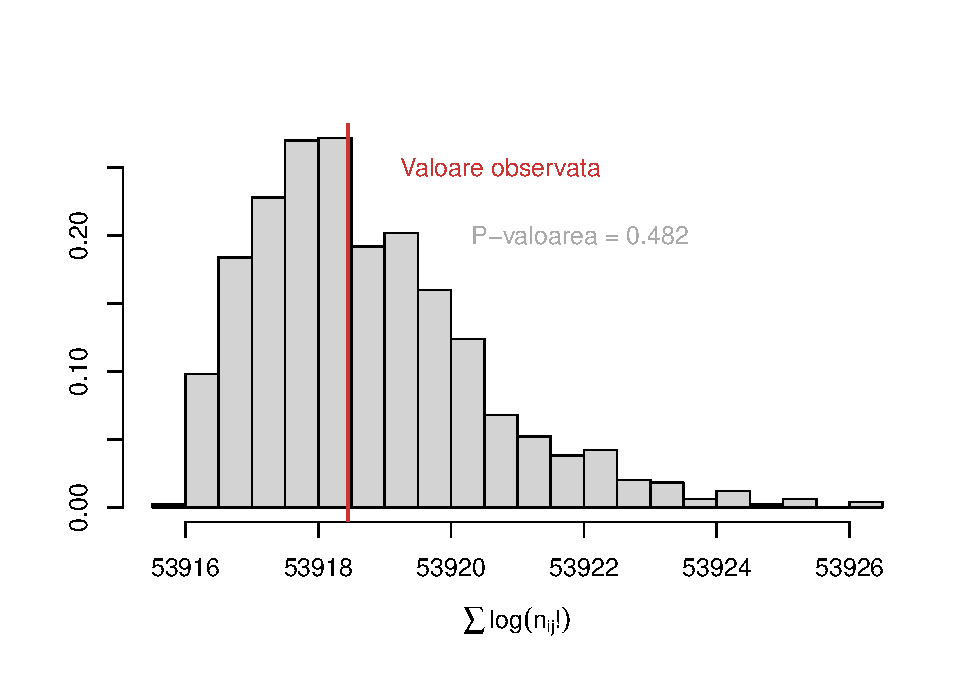
\includegraphics[width=0.9\linewidth]{Lab_3_files/figure-latex/unnamed-chunk-30-1} \end{center}

Același rezultat îl obținem și dacă folosim funcția \texttt{fisher.test}
(care este mai rapidă):

\begin{Shaded}
\begin{Highlighting}[]
\KeywordTok{fisher.test}\NormalTok{(matAA_observed, }\DataTypeTok{simulate.p.value =} \OtherTok{TRUE}\NormalTok{, }\DataTypeTok{B =} \DecValTok{1000}\NormalTok{)}
\end{Highlighting}
\end{Shaded}

\begin{verbatim}
## 
##  Fisher's Exact Test for Count Data with simulated p-value (based
##  on 1000 replicates)
## 
## data:  matAA_observed
## p-value = 0.4975
## alternative hypothesis: two.sided
\end{verbatim}


\end{document}
